\clearpairofpagestyles
% \renewcommand{\pagemark}{{\usekomafont{pagenumber}{Page \thepage\ of \pageref{LastPage}}}}
\renewcommand{\pagemark}{{\usekomafont{pagenumber}{ \thepage\ }}}
% \ohead*{\vspace{-1cm}BIT Camp 자바 177기 1조 왕밤빵 \hfill}
\ohead*{\vspace{-0.5cm}BIT Camp 자바 177기 1조 왕밤빵}
\ofoot*{\pagemark}
\pagenumbering{arabic}
\setcounter{page}{1} %%% This is only to be included in the first content file to restart the page numbers using a different format %%%

\hiddenchapter{프로젝트 개요}
\ChapterTitle[\thechapter]{프로젝트 개요}
%%% See Preamble for an explanation of both of these %%%

\hiddensection{시스템 개요}
\SectionTitle{\thesection}{시스템 개요} \\

\begin{adjustwidth}{0.45cm}{}
\subsection*{프로젝트 명}
\end{adjustwidth}
\begin{adjustwidth}{0.6cm}{}
\large{트래블 다이어리 (틀-다) A Travel Diary}
\normalsize
\end{adjustwidth}

\subsection{프로젝트 소개}
\begin{adjustwidth}{0.6cm}{}
\hspace{1em} 2020년 2월 말 이후 코로나 19 대유행으로 인해 해외는 물론 국내 여행도 떠나기 어려운 상황이 되어 여행 예약 서비스들의 수요가 하락하고 있는 추세이고, 코로나 19가 종식되지 않을 것이라고 예상되는 가까운 미래보다 코로나 19 이전의 삶을 추억하는 사람들이 늘어나고 있다. 하지만 현재 존재하는 여행 관련 웹 사이트들은 여행지의 소개나 숙소 예약 등 미래의 여행을 위한 사이트들이 다반사이며 과거의 여행을 추억하는 사이트는 찾아보기 어렵다. 따라서 본 프로젝트에서는 미래를 위한 여행 사이트가 아닌 이미 다녀온 과거 여행지의 추억을 회상하고 기록하며, 다른 사람들과 공유할 수 있는 사이트를 제공하고자 한다. 더 나아가서 커뮤니티를 통해 다른 사람들과 여행 정보를 공유하며 여행 계획을 세울 수도 있다. 
\end{adjustwidth}

\begin{itemize}
    \item \textbf{주요 타겟} : 연령 무관하며 과거의 여행을 기록하고 공유하고 싶은 사람
    \item \textbf{주요 대상} : 넘쳐나는 여행 사진들을 관리하는 것에 대한 어려움을 느낀 적이 있거나, 자신의 여행 사진과 기록들을 타인에게 공유하고 싶을 때 한 곳에 모여 있지 않아 찾는 것에 불편함을 느낀 적이 있는 사람 
    \item 원하는 형식으로 자유롭게 여행 기록
    \begin{itemize}
        \item[] 여행을 기록하는 공간을 제공한다. 다녀왔던 장소에 대한 사진을 올리면 기록된 위치정보를 기반으로 지도에 표시가 되어지고, 직접 지도에 표시 할 수도 있다. 블로그 형식으로 여행에 대한 기록을 자유롭게 써내려갈 수 있고 글과 함께 사진, 동영상, 해시태그, 후기 등을 추가할 수 있다. 개인적인 기록이지만 원한다면 공개로 설정해서 다른 사람들과 공유할 수 있다.
        위의 기능들을 통해 과거의 여행에 대해 추억하며 현재 가지 못하는 여행에 대한 아쉬움을 달랠 수 있다.
    \end{itemize}
    
    \item 관리하기 어려운 여행 사진들, 앨범 형식으로 정리
    \begin{itemize}
        \item[] 앨범 형식으로 여행 사진들을 저장하여 과거의 여행이 생각 날 때 마다 언제든지 쉽게 찾아볼 수 있고, 정리하기 어려워 여기저기 흩어져 있던 사진들도 한 눈에 모아볼 수 있다.
    \end{itemize}
    
    \item 나만 보기 아까운 기록들, 타인과 공유
    \begin{itemize}
        \item[] SNS에 있는 기능들을 접목시킨 커뮤니티를 통해, 타인의 기록을 스크랩하고 좋아요를 누를 수 있으며 팔로우 기능도 제공한다. 
    \end{itemize}
    \item 채팅을 통한 여행 정보 공유의 장 
    \begin{itemize}
        \item[] 회원 가입 시에 설정해 둔 현재 거주지와 관심 여행지가 채팅을 사용할 때 표시가 되어 어떤 지역을 여행 가고자 하는 사람이 그 지역에 거주하는 사람을 쉽게 알아보고 정보를 공유할 수 있다.
    \end{itemize}
\end{itemize}
\par\
\newpage

\hiddensection{업무영역}
\SectionTitle{\thesection}{업무영역}

\subsection{나의 계정에서 할 수 있는 것들}

\begin{itemize}
    \item 기록 (CRUD)
    \begin{enumerate}
        \item 지도에 표시
            \begin{itemize}
                \item[] 기록의 시작은 지도이다. 내가 갔던 여행지를 지도에 깃발과 색으로 표시할 수 있다. 깃발을 클릭하면 그 여행지의 기록을 확인 할 수 있다.
            \end{itemize}
        \item 카테고리 별 블로그 형식으로 (사진, 동영상, 글, 가계부, 기념품, 해시태그 등) 자유롭게
            \begin{itemize}
                \item[] 여행 기간을 기술하고, 카테고리를 선택한 후 사용자가 원하는 형식으로 사진과 글, 날씨, 음악 등을 자유롭게 추가해서 블로그 형식으로 기록할 수 있다. 카테고리는 여행, 맛집, 여행 음악 추천, 여행지 추천 등 다양하게 구성하여 여행지에 대한 기록만 할 수 있는 게 아니라 여행에서 파생된 하위 분야들도 기록 할 수 있게 한다. 기록당 여러 개의 해시태그를 남길 수 있어 추후 기록 검색 시에 편리하게 이용할 수 있다.
            \end{itemize}
        \item 공개 / 비공개 설정
            \begin{itemize}
                \item[] 사용자는 본인의 기록을 다른 사람들과 공유할지 말지를 선택할 수 있다. 공개로 설정한다면 검색결과에 노출되며 다른 사용자가 스크랩 할 수 있고 좋아요를 받을 수도 있다.
            \end{itemize}
    \end{enumerate}
\end{itemize}

\begin{itemize}
    \item 후기
        \begin{itemize}
            \item [] 정형화된 형식에 맞춰 사진을 첨부하면서 여행지의 어떤 장소나 맛집 등에 대해 자신이 평점을 매기고 그에 대한 감상을 간단히 써내려 갈 수 있다.
        \end{itemize}
\end{itemize}

\begin{itemize}
    \item 사진첩 (앨범 형식)
        \begin{itemize}
            \item [] 기록 부분에 올린 사진과 별개로 여행 사진을 보관할 수 있는 공간. 여행 단위(앨범)로 보관하는 기능을 지원한다.
        \end{itemize}
\end{itemize}

\subsection{커뮤니티에서 할 수 있는 것들}

\begin{itemize}
    \item 채팅
    \begin{itemize}
        \item [] 사는 곳과 관심 여행지를 설정 해 놓은 사용자들은 여행 정보 공유 목적을 기반으로 한 채팅이 가능하다. 사용자들은 오픈채팅방 형식으로 이루어지는 채팅을 통해 편리하게 소통 할 수 있다.
    \end{itemize}
\end{itemize}

\begin{itemize}
    \item 커뮤니티 활동 (좋아요, 공유하기, 구독 등)
    \begin{itemize}
        \item [] 마음에 드는 기록이 있다면 좋아요를 누를 수 있고, 내 계정에 추가하고 싶은 기록이 있다면 스크랩을 하여 가져올 수 있으며 내용 수정과 추가도 가능하다. URL을 생성하여 SNS에 각 기록들을 공유할 수도 있다. 팔로우 기능을 통해 특정 사용자를 팔로우 하는 경우 그 사용자의 공개기록을 내 계정에서 열람할 수 있다.
    \end{itemize}
\end{itemize}

\subsection{개인 계정 관련}

\begin{itemize}
    \item 개인 정보 (사는 곳, 관심 지역 등) 
\end{itemize}

\begin{itemize}
    \item 회원 관리
    \begin{enumerate}
        \item 로그인, 로그아웃, 회원 정보 수정, 회원 탈퇴
        \begin{itemize}
            \item[] 사이트에 접속하기 위한 기초적인 로그인/아웃 시스템. 정보 업데이트와 더불어 더 이상 사이트에 개인정보를 남기고 싶지 않을 경우 탈퇴가 가능하다.
        \end{itemize}
    \end{enumerate}
\end{itemize}
\par\

\subsection{검색}

\begin{enumerate}
    \item 통합 검색
        \begin{itemize}
            \item[] 커뮤니티에서 이루어지는 검색과 개인 계정에서 이루어지는 검색을 분리한다.
            \item[] 검색 조건 : 제목, 해시태그, 장소, 내용, 제목+내용
            \item[] 검색 조건 입력 후 검색 시 분류가 된다. (전체, 이미지, 동영상, 후기 등)
        \end{itemize}
    \item 나의 계정에서 내 기록만 검색
        \begin{itemize}
            \item[] 개인 페이지에서 검색을 하면 ‘개인이 작성한 기록’만 나오도록 한다. 검색 결과는 개인이 설정해 놓은 공개 / 비공개와 상관 없이 등록한 모든 기록
        \end{itemize}
    \item 커뮤니티 통합 검색
        \begin{itemize}
            \item[] 커뮤니티 검색은 게시판에 올라온 ‘모든 글’을 검색한다. 공통 검색에 작성한 조건 외에 사용자 아이디나 닉네임 검색이 추가된다.
        \end{itemize}
\end{enumerate}


\subsection{기타}

\begin{itemize}
    \item 관리자 권한
        \begin{enumerate}
            \item 사용자 계정 정지
                \begin{itemize}
                    \item[] 사이트를 어지럽히는 행위(중복된 글을 도배하거나 욕설 및 비방 글 작성)을 일삼는 사용자들을 재재할 수 있다. 관리자는 금지어를 설정하고 그에 따라 사용자를 정지시키는 권한을 가진다.
                \end{itemize}
        \end{enumerate}
\end{itemize}
\par\
\newpage


\hiddensection{예상효과}
\SectionTitle{\thesection}{예상효과}

\begin{itemize}
    \item \textbf{여행의 추억 회상}
    \begin{itemize}
        \item [] 현재는 코로나19로 인해 여행을 직접 떠나기 힘들어졌고 앞으로도 이런 상황이 얼마나 더 지속될지 알 수 없다. 과거 여행지에서 느꼈던 감정과 기억들을 되짚어 나가면서 천천히 글을 써 내려가는 동안 사용자들은  추억을 되새겨 볼 수 있으며 언제든지 생각 날 때 마다 쉽게 꺼내 볼 수 있다.
    \end{itemize}
\end{itemize}

\begin{itemize}
    \item \textbf{효율적인 기록 관리}
    \begin{itemize}
        \item [] 사진을 글과 함께 기록하고 여행 경로도 알 수 있으니 기억에 의존하는 것보다 여행 당시 기분을 보다 생생하게 남길 수 있다. 여행 단위로 기록이 보관되며 사진만 따로 보관할 수 있는 앨범도 지원하기에 관리하기 용이해진다.
    \end{itemize}
\end{itemize}

\begin{itemize}
    \item \textbf{커뮤니티를 통한 여행 정보 공유}
    \begin{itemize}
        \item [] 커뮤니티를 이용해 다른 사람의 공개된 여행 기록을 열람하여 그 여행지에 대해 간접적으로 체험할 수 있다. 오픈 채팅방을 통해 관심있는 여행지의 현지인이나 여행을 다녀온 사람들에게 여행지에 관한 정보들을 서로 나눌 수 있게 된다.
    \end{itemize}
\end{itemize}
\par\

\begin{tcolorbox}
    종합해 보자면, 사용자들은 본 사이트를 통해 과거 여행지에 대한 추억을 회상할 수 있고 다른 사용자들의 기록들도 보며 식견을 넓힐 수 있다. 상대적으로 많은 사람들이 관심 있어 하는 여행이라는 카테고리로 범주를 좁혀놓았을 뿐, 개인의 생각이나 경험을 공유하고 타인과의 관계도 생성할 수 있는 개방화된 하나의 소셜 미디어, 온라인 플랫폼으로 볼 수 있어 엔드유저의 입장에서 사이트에 대한 접근성도 높을 것이라 예상된다.
\end{tcolorbox}

\newpage

\hiddensection{기술적 고려사항}
\SectionTitle{\thesection}{기술적 고려사항}

\begin{enumerate}
    \item 적용 방법론
        \begin{itemize}
            \item 객체 지향 설계 기법
                \begin{itemize}
                    \item[] 책임-주도 설계
                    \item[] 디자인 패턴
                    \item[] 테스트-주도 개발
                \end{itemize}
        \end{itemize}
        \begin{itemize}
            \item 모델링
                \begin{itemize}
                    \item[] 유스케이스
                    \item[] 도메인
                \end{itemize}
        \end{itemize}
    \item Architecture
        \begin{itemize}
            \item 2 Layer Architecture
            \item MVC Model 2 Architecture
            \item Interface-based programming
        \end{itemize}
    \item Framework
        \begin{itemize}
            \item{} [ Back-End ]
                \begin{itemize}
                    \item[] Servlet \& Jsp
                    \item[] Spring Framework
                    \item[] Express.js
                \end{itemize}
            \item{} [ Front-End ]
                \begin{itemize}
                    \item[] jQuery
                    \item[] React.js
                    \item[] Bootstrap 4
                    \item[] Summernote
                \end{itemize}
            \item{} [ Database ]
                \begin{itemize}
                    \item[] MyBatis
                \end{itemize}
        \end{itemize}
    \item 적용 기술
        \begin{itemize}
            \item Java 
            \item HTML5/CSS3
            \item Javascript
            \item Node.js
            \item JSON
            \item Ajax
            \item JSTL
            \item EL
            \item Oracle 11g
        \end{itemize}

    \item 기술적 특이사항 
    \begin{itemize}
        \item{} [ Open API 사용 ]
            \begin{itemize}
                \item[] Google Map API
            \end{itemize}
    \end{itemize}
\end{enumerate}
\par\
\newpage

\hiddensection{개발이력}
\SectionTitle{\thesection}{개발이력}

\begin{enumerate}
    \item 개발 기간 10주 (2020.12.14 ~ 2020.02.22)
        \begin{itemize}
            \item 분석, 설계 : 4주
            \item 구현 : 5주
            \item 보고서 작성 및 발표 준비 : 1주
        \end{itemize}

        \begin{figure}[h]
            \begin{center}
                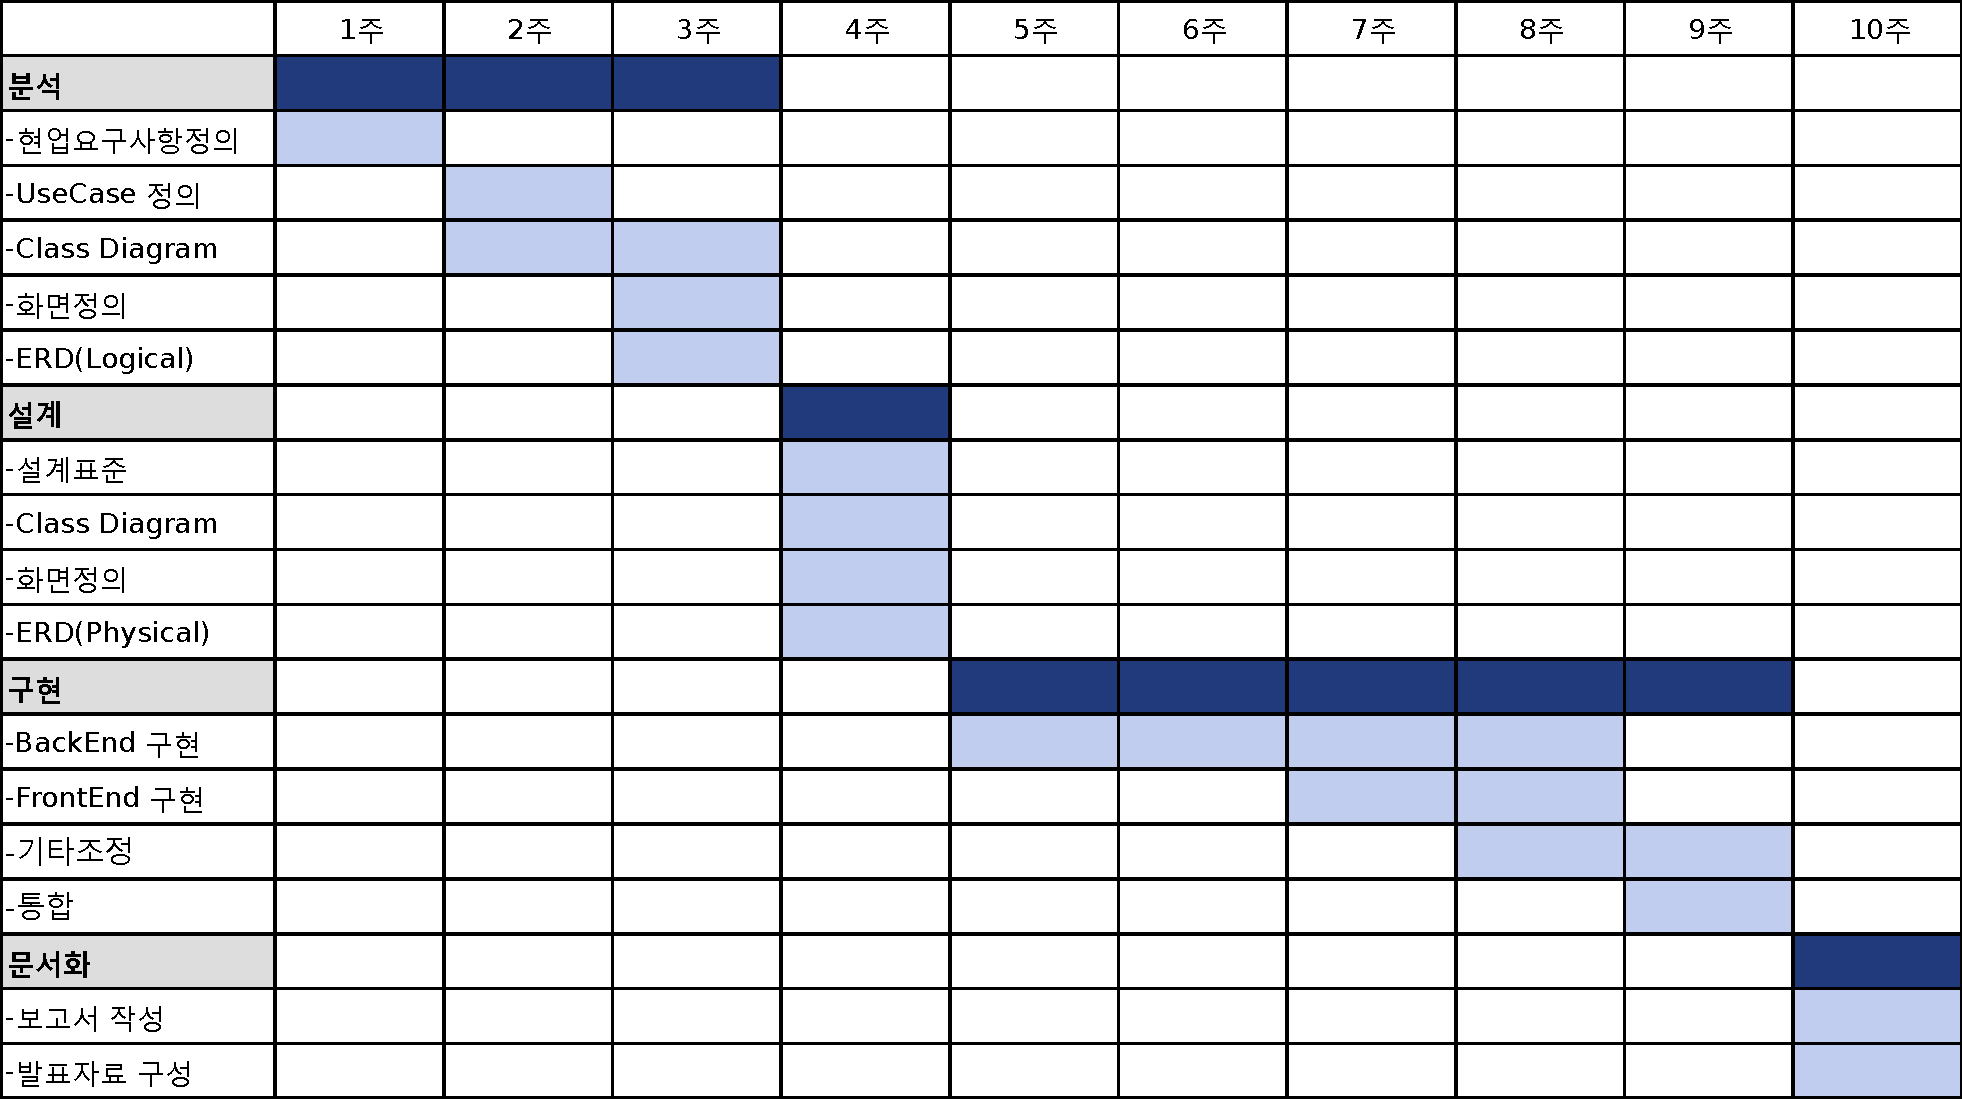
\includegraphics[width=16cm]{./Figure/devel.pdf}
            \end{center}
        \end{figure}


    \item 기능별 역할 분담
        \begin{itemize}
            \item[] [ 공통 역할 ] 
                \begin{itemize}
                    \item[] Content 기획, Web 기획 및 개발, DB 설계 및 구현, 화면 구성
                \end{itemize}
            \item[] [ 세부 역할 ]
            
            \begin{tabular}{ |p{2cm}|p{12cm}| }
                \hline
                \textbf{성 명} & \textbf{역할} \\
                \hline
                정주원 & GoogleMap API, summernote를 이용한 기록 등록 등 기록 CRUD / 통합검색 시 해시태그별, 기록별 검색 / 메인페이지에 보여지는 top10 관리 / 북마크 보조 \\
                \hline
                김성영 & Node.js, Express.js, React.js를 이용한 채팅시스템 / 후기 CRUD와 평점등록 / 회원 구독을 통한 기록 조회 / 통합검색 시 후기별 검색 \\
                \hline
                김채경 & 회원, 관리자 권한 분리 / 회원 CRUD / 블랙리스트 관리 / 통합검색 시 회원별 검색 \\
                \hline
                박정인 & 앨범 형식의 사진 관리 / 회원관리 보조 / 다중파일 업로드 기반 사진 등록 \\
                \hline
                임제현 & summernote를 이용한 자유게시판 CRUD /  북마크 추가, 삭제 및 조회 \\
                \hline
            \end{tabular}

        \end{itemize}
    \newpage
    \item 개발 환경 구축
    \begin{itemize}
        \item S/W 
            \begin{itemize}
                \item[] OS : Window / Mac OS
            \end{itemize}
        \item Tool
        \begin{itemize}
            \item[] IDE : Eclipse, Visual Studio Code
            \item[] DB : Oracle Database
            \item[] WAS : Apache Tomcat 8.5
            \item[] JDK : 1.8
            \item[] 형상관리 : Git Hub
        \end{itemize}
    \end{itemize}

\end{enumerate}
\par\
% \newpage

\hiddensection{Web Application Architecture}
\SectionTitle{\thesection}{Web Application Architecture}

\begin{figure}[h]
    \begin{center}
        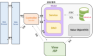
\includegraphics[width=16cm]{./Figure/Model2MVC.pdf}
    \end{center}
\end{figure}
\newpage